\documentclass[border=5pt]{standalone}
\usepackage{tikz}
\usetikzlibrary{arrows.meta, positioning, decorations.pathreplacing, calc, shapes.geometric}
\usepackage{xcolor}

\definecolor{Garnet}{HTML}{73000A}
\definecolor{NinetyBlack}{HTML}{363636}
\definecolor{SeventyBlack}{HTML}{5C5C5C}
\definecolor{FiftyBlack}{HTML}{A2A2A2}
\definecolor{ThirtyBlack}{HTML}{C7C7C7}
\definecolor{TenBlack}{HTML}{ECECEC}
\definecolor{Atlantic}{HTML}{466A9F}
\definecolor{Rose}{HTML}{CC2E40}
\definecolor{Congaree}{HTML}{1F414D}
\definecolor{Sandstorm}{HTML}{FFF2E3}

\tikzset{every node/.append style={rounded corners=0pt}}

\begin{document}
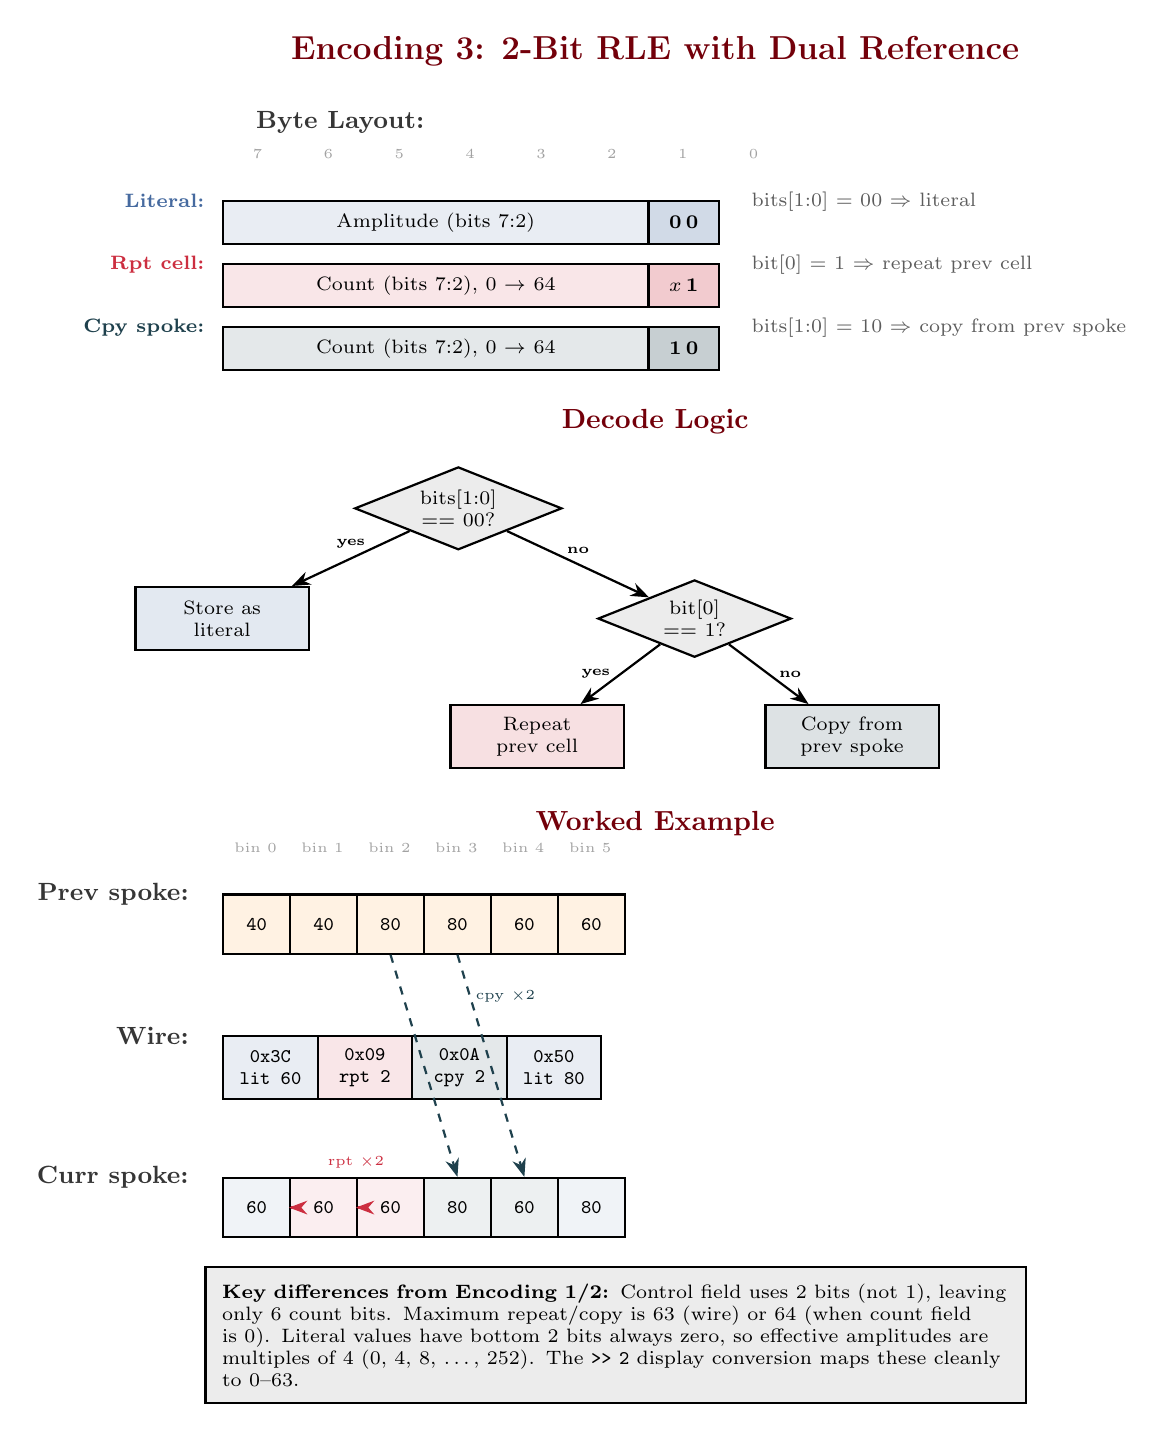
\begin{tikzpicture}[
    cell/.style={draw, thick, minimum width=1.2cm, minimum height=0.8cm, anchor=west, font=\ttfamily\scriptsize, align=center},
    scell/.style={draw, thick, minimum width=0.85cm, minimum height=0.75cm, anchor=west, font=\ttfamily\scriptsize, align=center},
    lbl/.style={font=\small\bfseries, color=NinetyBlack},
    annot/.style={font=\scriptsize, color=SeventyBlack},
    decision/.style={draw, thick, diamond, aspect=2.5, minimum width=2cm, font=\scriptsize, align=center, inner sep=2pt},
]

\node[font=\bfseries\large, color=Garnet] at (5.5, 7.5) {Encoding 3: 2-Bit RLE with Dual Reference};

% ── Byte layout with 2-bit control ──
\node[lbl] at (1.5, 6.6) {Byte Layout:};

% Bit positions
\foreach \i/\v in {0/7, 1/6, 2/5, 3/4, 4/3, 5/2, 6/1, 7/0} {
    \node[font=\tiny, color=FiftyBlack] at (0.45 + \i*0.9, 6.2) {\v};
}

% Show the 3 modes
\node[font=\scriptsize\bfseries, color=Atlantic, anchor=east] at (-0.1, 5.6) {Literal:};
\node[draw, thick, fill=Atlantic!12, minimum width=5.4cm, minimum height=0.55cm, anchor=west, font=\scriptsize] at (0, 5.33) {Amplitude (bits 7:2)};
\node[draw, thick, fill=Atlantic!25, minimum width=0.9cm, minimum height=0.55cm, anchor=west, font=\scriptsize\bfseries] at (5.4, 5.33) {0\,0};
\node[annot, anchor=west] at (6.6, 5.6) {bits[1:0] = 00 $\Rightarrow$ literal};

\node[font=\scriptsize\bfseries, color=Rose, anchor=east] at (-0.1, 4.8) {Rpt cell:};
\node[draw, thick, fill=Rose!12, minimum width=5.4cm, minimum height=0.55cm, anchor=west, font=\scriptsize] at (0, 4.53) {Count (bits 7:2), 0 $\rightarrow$ 64};
\node[draw, thick, fill=Rose!25, minimum width=0.9cm, minimum height=0.55cm, anchor=west, font=\scriptsize\bfseries] at (5.4, 4.53) {$x$\,1};
\node[annot, anchor=west] at (6.6, 4.8) {bit[0] = 1 $\Rightarrow$ repeat prev cell};

\node[font=\scriptsize\bfseries, color=Congaree, anchor=east] at (-0.1, 4.0) {Cpy spoke:};
\node[draw, thick, fill=Congaree!12, minimum width=5.4cm, minimum height=0.55cm, anchor=west, font=\scriptsize] at (0, 3.73) {Count (bits 7:2), 0 $\rightarrow$ 64};
\node[draw, thick, fill=Congaree!25, minimum width=0.9cm, minimum height=0.55cm, anchor=west, font=\scriptsize\bfseries] at (5.4, 3.73) {1\,0};
\node[annot, anchor=west] at (6.6, 4.0) {bits[1:0] = 10 $\Rightarrow$ copy from prev spoke};

% ── Decision flowchart ──
\node[font=\bfseries, color=Garnet] at (5.5, 2.8) {Decode Logic};

\node[decision, fill=TenBlack] (d1) at (3.0, 1.7) {bits[1:0]\\== 00?};
\node[draw, thick, fill=Atlantic!15, minimum width=2.2cm, minimum height=0.8cm, font=\scriptsize, align=center] (lit) at (0, 0.3) {Store as\\literal};
\node[decision, fill=TenBlack] (d2) at (6.0, 0.3) {bit[0]\\== 1?};
\node[draw, thick, fill=Rose!15, minimum width=2.2cm, minimum height=0.8cm, font=\scriptsize, align=center] (rpt) at (4.0, -1.2) {Repeat\\prev cell};
\node[draw, thick, fill=Congaree!15, minimum width=2.2cm, minimum height=0.8cm, font=\scriptsize, align=center] (cpy) at (8.0, -1.2) {Copy from\\prev spoke};

\draw[-{Stealth}, thick] (d1) -- (lit) node[midway, above, font=\tiny\bfseries] {yes};
\draw[-{Stealth}, thick] (d1) -- (d2) node[midway, above, font=\tiny\bfseries] {no};
\draw[-{Stealth}, thick] (d2) -- (rpt) node[midway, left, font=\tiny\bfseries] {yes};
\draw[-{Stealth}, thick] (d2) -- (cpy) node[midway, right, font=\tiny\bfseries] {no};

% ── Worked Example ──
\node[font=\bfseries, color=Garnet] at (5.5, -2.3) {Worked Example};

% Previous spoke
\node[lbl, anchor=east] at (-0.3, -3.2) {Prev spoke:};
\node[scell, fill=Sandstorm] (p0) at (0, -3.58) {40};
\node[scell, fill=Sandstorm] (p1) at (0.85, -3.58) {40};
\node[scell, fill=Sandstorm] (p2) at (1.7, -3.58) {80};
\node[scell, fill=Sandstorm] (p3) at (2.55, -3.58) {80};
\node[scell, fill=Sandstorm] (p4) at (3.4, -3.58) {60};
\node[scell, fill=Sandstorm] (p5) at (4.25, -3.58) {60};

\foreach \i in {0,...,5} {
    \node[font=\tiny, color=FiftyBlack, above=1pt] at (0.425 + \i*0.85, -2.83) {bin \i};
}

% Wire bytes
\node[lbl, anchor=east] at (-0.3, -5.0) {Wire:};
\node[cell, fill=Atlantic!12] (w0) at (0, -5.4) {\texttt{0x3C}\\lit 60};
\node[cell, fill=Rose!12] (w1) at (1.2, -5.4) {\texttt{0x09}\\rpt 2};
\node[cell, fill=Congaree!12] (w2) at (2.4, -5.4) {\texttt{0x0A}\\cpy 2};
\node[cell, fill=Atlantic!12] (w3) at (3.6, -5.4) {\texttt{0x50}\\lit 80};

% Current spoke
\node[lbl, anchor=east] at (-0.3, -6.8) {Curr spoke:};
\node[scell, fill=Atlantic!8] (c0) at (0, -7.18) {60};
\node[scell, fill=Rose!8] (c1) at (0.85, -7.18) {60};
\node[scell, fill=Rose!8] (c2) at (1.7, -7.18) {60};
\node[scell, fill=Congaree!8] (c3) at (2.55, -7.18) {80};
\node[scell, fill=Congaree!8] (c4) at (3.4, -7.18) {60};
\node[scell, fill=Atlantic!8] (c5) at (4.25, -7.18) {80};

\foreach \i in {0,...,5} {
    \node[font=\tiny, color=FiftyBlack, below=1pt] at (0.425 + \i*0.85, -7.93) {bin \i};
}

% Horizontal arrows (repeat previous cell)
\draw[-{Stealth}, thick, Rose, dashed] (c0.east) -- (c1.west);
\draw[-{Stealth}, thick, Rose, dashed] (c1.east) -- (c2.west);
\node[font=\tiny, color=Rose] at (1.7, -6.6) {rpt $\times 2$};

% Vertical arrows (copy from previous spoke)
\draw[-{Stealth}, thick, Congaree, dashed] ($(p2.south)$) -- ($(c3.north)$);
\draw[-{Stealth}, thick, Congaree, dashed] ($(p3.south)$) -- ($(c4.north)$);
\node[font=\tiny, color=Congaree] at (3.6, -4.5) {cpy $\times 2$};

% Note
\node[draw, thick, fill=TenBlack, text width=10cm, align=left, font=\scriptsize, inner sep=6pt] at (5.0, -8.8)
    {\textbf{Key differences from Encoding 1/2:} Control field uses 2 bits (not 1), leaving only 6 count bits. Maximum repeat/copy is 63 (wire) or 64 (when count field is 0). Literal values have bottom 2 bits always zero, so effective amplitudes are multiples of 4 (0, 4, 8, \ldots, 252). The \texttt{>> 2} display conversion maps these cleanly to 0--63.};

\end{tikzpicture}
\end{document}
